\documentclass[11pt,a4paper]{article}

% --- Encoding / layout (pdflatex-safe) ---
\usepackage[utf8]{inputenc}
\usepackage[T1]{fontenc}
\usepackage[a4paper,margin=22mm]{geometry}
\usepackage{amsmath,amssymb}
\usepackage{booktabs}
\usepackage{array}
\usepackage{enumitem}
\usepackage{graphicx}
\usepackage{float}
\usepackage{caption}
\usepackage{xcolor} % only black/white used
\usepackage[hidelinks]{hyperref}
\usepackage{listings}

% --- TikZ (B/W only) ---
\usepackage{tikz}
\usetikzlibrary{shapes.geometric,arrows.meta,positioning,fit,calc}

\tikzset{
  bwbox/.style={rectangle, draw=black, fill=white, thick, minimum width=28mm, minimum height=10mm, align=center, font=\small},
  bwboxwide/.style={rectangle, draw=black, fill=white, thick, minimum width=38mm, minimum height=10mm, align=center, font=\small},
  bwheader/.style={rectangle, draw=black, fill=black, text=white, thick, minimum width=28mm, minimum height=8mm, align=center, font=\small\bfseries},
  bwdata/.style={cylinder, draw=black, fill=white, thick, shape border rotate=90, aspect=0.25, minimum width=22mm, minimum height=10mm, align=center, font=\small},
  bwdecision/.style={diamond, draw=black, fill=white, thick, aspect=2, align=center, font=\small, inner sep=2pt},
  bwarrow/.style={-{Latex[length=2.5mm]}, thick, draw=black},
  bwline/.style={thick, draw=black},
  bwdashed/.style={thick, draw=black, dashed, -{Latex[length=2.5mm]}},
}

\lstset{
  basicstyle=\footnotesize\ttfamily,
  frame=single,
  rulecolor=\color{black},
  backgroundcolor=\color{white},
  keywordstyle=\bfseries,
  commentstyle=\itshape,
  showstringspaces=false,
  breaklines=true,
  tabsize=2
}

\title{UmbraCrawl\\Stealth Web Crawling Framework --- Architecture Research Document}
\author{Source survey: Scrapling, Crawlee, Scrapy, Colly, Camoufox, Patchright, undetected-chromedriver, Crawl4AI, Firecrawl}
\date{2026-10-10}

\begin{document}
\maketitle
\begin{center}
\begin{minipage}{0.92\textwidth}
\small\textbf{Scope.} UmbraCrawl design for a new stealthy crawler combining HTTP impersonation, engine-level anti-detect browsers, adaptive parsing, and production orchestration. Monochrome edition: all 21 figures use black lines on white only. Sources are the ten cloned repositories listed in Section~2.
\end{minipage}
\end{center}
\tableofcontents
\newpage

% ============================================================
\section{Goals and Threat Model}
% ============================================================
\subsection{Goals}
\begin{enumerate}[leftmargin=*,itemsep=2pt]
\item Crawl clear and bot-protected targets with one router: fast HTTP path by default, browser path only on challenge.
\item Keep ban rate low via session isolation, proxy health tracking, and per-profile fingerprint consistency.
\item Survive layout drift via multi-candidate selectors with scoring and auto-relearn snapshots.
\item Emit dual outputs: validated item JSON and LLM-ready Markdown.
\item Operate as a queue of workers with observable metrics: requests/s, challenge rate, leak score, parse recall.
\end{enumerate}

\subsection{Threat model}
Adversaries: Cloudflare, DataDome, Imperva, PerimeterX / Human, Akamai. Signals they use:
\begin{enumerate}[leftmargin=*,itemsep=2pt]
\item Network: TLS ClientHello fingerprint (JA3), HTTP/2 SETTINGS order, header order and casing.
\item Runtime: \texttt{navigator.webdriver}, CDP command artifacts, missing browser plugins, WebGL renderer strings.
\item Behaviour: instant navigation, no mouse/scroll, fixed viewport, datacenter ASN, cookie reuse across identities.
\item Content: honeypot links, obfuscated class names, JS-required bodies.
\end{enumerate}
Design rule: any identity (session + proxy + fingerprint) is used consistently for its lifetime and retired on challenge failure, never mixed.

% ============================================================
\section{Source Survey: What Is Taken From Each Repository}
% ============================================================
All repositories were cloned shallow on 2026-10-10 into the working directory. Table~\ref{tab:borrow} summarises reuse.

\begin{table}[H]
\centering
\caption{Reuse matrix. Take = port the pattern; Leave = consume as dependency or discard.}
\label{tab:borrow}
\begin{tabular}{@{}p{3.2cm}p{5.2cm}p{5.2cm}@{}}
\toprule
Repo (local dir) & Take & Leave \\
\midrule
D4Vinci-Scrapling \newline \texttt{scrapling/fetchers/, parser.py} &
Fetcher router HTTP $\rightarrow$ impersonate $\rightarrow$ browser; adaptive selector scoring; \texttt{curl\_cffi} + \texttt{browserforge} usage. &
Spider/CLI wrapper; reimplement scheduler interface. \\
apify/crawlee-python \newline \texttt{src/crawlee/} &
SessionPool, ProxyConfiguration, RequestQueue dedupe, AutoscalingPool, Router table. &
SQLite-backed clients; same interfaces, local files. \\
apify/crawlee JS \newline \texttt{packages/browser-pool/} &
Browser retire/relaunch policy; per-page injection hooks; header ordering from \texttt{got-scraping-client}. &
Node transports; port to \texttt{asyncio}. \\
scrapy/scrapy \newline \texttt{core/, middlewares/} &
Middleware chain, politeness, \texttt{dupefilters.py}, LinkExtractor rules, Settings priorities, feed exports. &
Twisted engine; rebuild on \texttt{asyncio}. \\
gocolly/colly \newline \texttt{colly.go, queue/} &
\texttt{OnRequest/OnHTML/OnResponse} callbacks; throttling queue; \texttt{unmarshal.go} struct mapping. &
Go runtime; HTTP-only limits. \\
daijro/camoufox \newline \texttt{pythonlib/camoufox/} &
Engine-level fingerprint model, locale/font/viewport presets, WebGL/canvas addons, launch args. &
Build system (\texttt{multiversion.py}); use as dependency. \\
Kaliiiiiiiiii-Vinyzu/patchright \newline \texttt{patchright.patch} &
CDP leak patch list; driver patch method; \texttt{detection\_smoke\_test.mjs} as regression template. &
Fork maintenance; consume patched driver. \\
ultrafunkamsterdam/undetected-chromedriver &
Patch-point reference (\texttt{patcher.py}, \texttt{cdp.py}) only. &
Runtime (stale 2025-07-05); Selenium blocking model. \\
unclecode/crawl4ai &
Dispatcher fan-out; Markdown generation, content filter, chunking; \texttt{async\_configs.py} knobs. &
Monolithic crawler class; split into stages. \\
mendableai/firecrawl \newline \texttt{apps/api/} &
Local run shape (prompt $\rightarrow$ crawl $\rightarrow$ cited answer); scraper/service boundary; single-SQLite storage pattern. &
Server stack (Redis, Postgres, SDK fleet); local CLI replaces the gateway. \\
\bottomrule
\end{tabular}
\end{table}

% ============================================================
\section{System Architecture}
% ============================================================
Figure~\ref{fig:layers} shows the layered view. Every request passes through identity binding before any network I/O.

\begin{figure}[H]
\centering
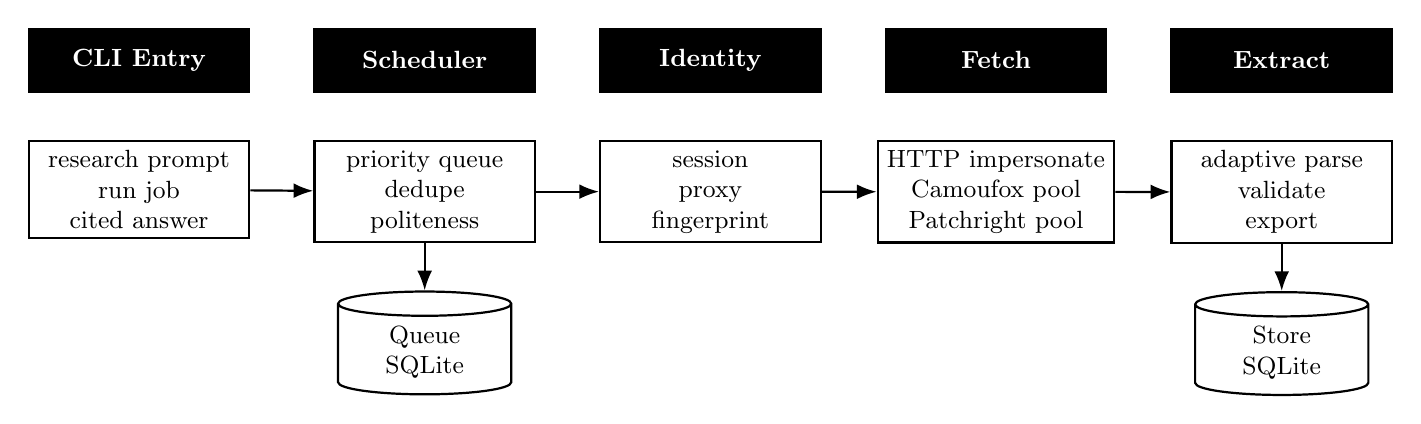
\begin{tikzpicture}[node distance=6mm and 8mm]
\node[bwheader] (api) {CLI Entry};
\node[bwheader, right=of api] (sched) {Scheduler};
\node[bwheader, right=of sched] (ident) {Identity};
\node[bwheader, right=of ident] (fetch) {Fetch};
\node[bwheader, right=of fetch] (parse) {Extract};
\node[bwbox, below=of api] (api1) {research prompt\\run job\\cited answer};
\node[bwbox, below=of sched] (sched1) {priority queue\\dedupe\\politeness};
\node[bwbox, below=of ident] (ident1) {session\\proxy\\fingerprint};
\node[bwbox, below=of fetch] (fetch1) {HTTP impersonate\\Camoufox pool\\Patchright pool};
\node[bwbox, below=of parse] (parse1) {adaptive parse\\validate\\export};
\node[bwdata, below=of sched1] (q) {Queue\\SQLite};
\node[bwdata, below=of parse1] (db) {Store\\SQLite};
\draw[bwarrow] (api1) -- (sched1);
\draw[bwarrow] (sched1) -- (ident1);
\draw[bwarrow] (ident1) -- (fetch1);
\draw[bwarrow] (fetch1) -- (parse1);
\draw[bwarrow] (sched1) -- (q);
\draw[bwarrow] (parse1) -- (db);
\end{tikzpicture}
\caption{Layered architecture. Identity binding precedes fetch; storage is behind the pipeline, never beside it.}
\label{fig:layers}
\end{figure}

\subsection{Component responsibilities}
\begin{table}[H]
\centering
\caption{Module contract summary.}
\begin{tabular}{@{}p{3.4cm}p{5cm}p{5.2cm}@{}}
\toprule
Module & Input $\rightarrow$ Output & Failure mode \\
\midrule
\texttt{cli/} & Prompt $\rightarrow$ cited answer rows & Reject empty prompt, no crawl started. \\
\texttt{scheduler/} & URLs $\rightarrow$ leased tasks & Drop duplicates, backoff per-host. \\
\texttt{identity/} & Task $\rightarrow$ bound (session, proxy, profile) & Retire identity on 2 challenges. \\
\texttt{fetchers/} & Bound task $\rightarrow$ raw response & Escalate HTTP $\rightarrow$ browser, else poison. \\
\texttt{parser/} & HTML $\rightarrow$ items + Markdown & Snapshot + relearn on zero-match. \\
\texttt{pipeline/} & Raw items $\rightarrow$ clean rows & Quarantine on schema fail. \\
\bottomrule
\end{tabular}
\end{table}

Proposed file tree:
\begin{lstlisting}
umbracrawl/
  cli/            prompt.py, run.py, answer.py
  scheduler/    queue.py, politeness.py, dedupe.py
  identity/     sessions.py, proxies.py, fingerprints.py, leakcheck.py
  fetchers/     http_impersonate.py, camoufox_pool.py,
                patchright_pool.py, router.py
  parser/       adaptive.py, selectors.yml, markdown.py
  pipeline/     validate.py, clean.py, export.py
  storage/      sqlite.py (tasks, items, identities; FTS5)
  observability/ metrics.py, traces.py
  tests/        leak_suite.py, challenge_fixtures/
\end{lstlisting}

% ============================================================
\section{Flow 1: Fetch Escalation}
% ============================================================
Figure~\ref{fig:escalation} is the core cost saver: the cheap path handles clear targets, the browser path handles only challenges.

\begin{figure}[H]
\centering
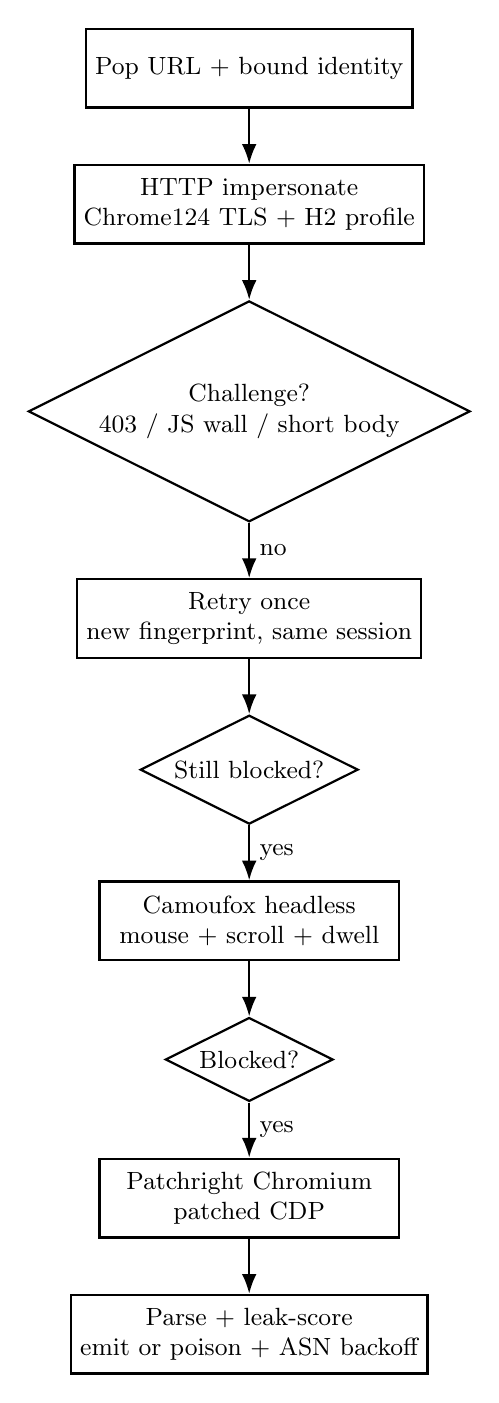
\begin{tikzpicture}[node distance=7mm]
\node[bwboxwide] (a) {Pop URL + bound identity};
\node[bwboxwide, below=of a] (b) {HTTP impersonate\\Chrome124 TLS + H2 profile};
\node[bwdecision, below=of b] (c) {Challenge?\\403 / JS wall / short body};
\node[bwboxwide, below=of c] (d) {Retry once\\new fingerprint, same session};
\node[bwdecision, below=of d] (e) {Still blocked?};
\node[bwboxwide, below=of e] (f) {Camoufox headless\\mouse + scroll + dwell};
\node[bwdecision, below=of f] (g) {Blocked?};
\node[bwboxwide, below=of g] (h) {Patchright Chromium\\patched CDP};
\node[bwboxwide, below=of h] (i) {Parse + leak-score\\emit or poison + ASN backoff};
\draw[bwarrow] (a) -- (b);
\draw[bwarrow] (b) -- (c);
\draw[bwarrow] (c) -- node[right,font=\small]{no} (d);
\draw[bwarrow] (d) -- (e);
\draw[bwarrow] (e) -- node[right,font=\small]{yes} (f);
\draw[bwarrow] (f) -- (g);
\draw[bwarrow] (g) -- node[right,font=\small]{yes} (h);
\draw[bwarrow] (h) -- (i);
\end{tikzpicture}
\caption{Fetch escalation. Browser stages execute only after HTTP fails twice.}
\label{fig:escalation}
\end{figure}

Rules: maximum two HTTP attempts per identity; browser stages reuse the same proxy so behaviour stays consistent; three consecutive browser failures poison the URL and cool down the ASN.

% ============================================================
\section{Flow 2: Stealth Handshake}
% ============================================================
Figure~\ref{fig:handshake} shows identity binding order. Order matters: fingerprint first, then proxy, then network.

\begin{figure}[H]
\centering
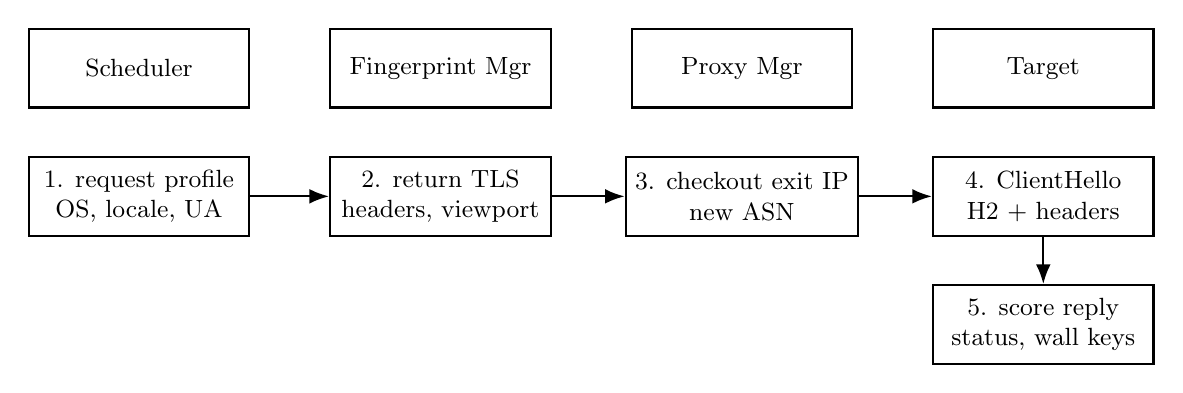
\begin{tikzpicture}[node distance=6mm and 10mm]
\node[bwbox] (s) {Scheduler};
\node[bwbox, right=of s] (f) {Fingerprint Mgr};
\node[bwbox, right=of f] (p) {Proxy Mgr};
\node[bwbox, right=of p] (t) {Target};
\node[bwbox, below=of s] (s1) {1. request profile\\OS, locale, UA};
\node[bwbox, below=of f] (f1) {2. return TLS\\headers, viewport};
\node[bwbox, below=of p] (p1) {3. checkout exit IP\\new ASN};
\node[bwbox, below=of t] (t1) {4. ClientHello\\H2 + headers};
\node[bwbox, below=of t1] (t2) {5. score reply\\status, wall keys};
\draw[bwarrow] (s1) -- (f1);
\draw[bwarrow] (f1) -- (p1);
\draw[bwarrow] (p1) -- (t1);
\draw[bwarrow] (t1) -- (t2);
\end{tikzpicture}
\caption{Handshake order. No request leaves without a bound triple (session, proxy, profile).}
\label{fig:handshake}
\end{figure}

Consistency checklist per identity: same User-Agent and Sec-CH-UA across redirects; same viewport and timezone; same exit IP for the session lifetime; cookies isolated per session file.

% ============================================================
\section{Flow 3: Adaptive Parsing}
% ============================================================
Figure~\ref{fig:parser} covers layout drift, the Scrapling-derived stage.

\begin{figure}[H]
\centering
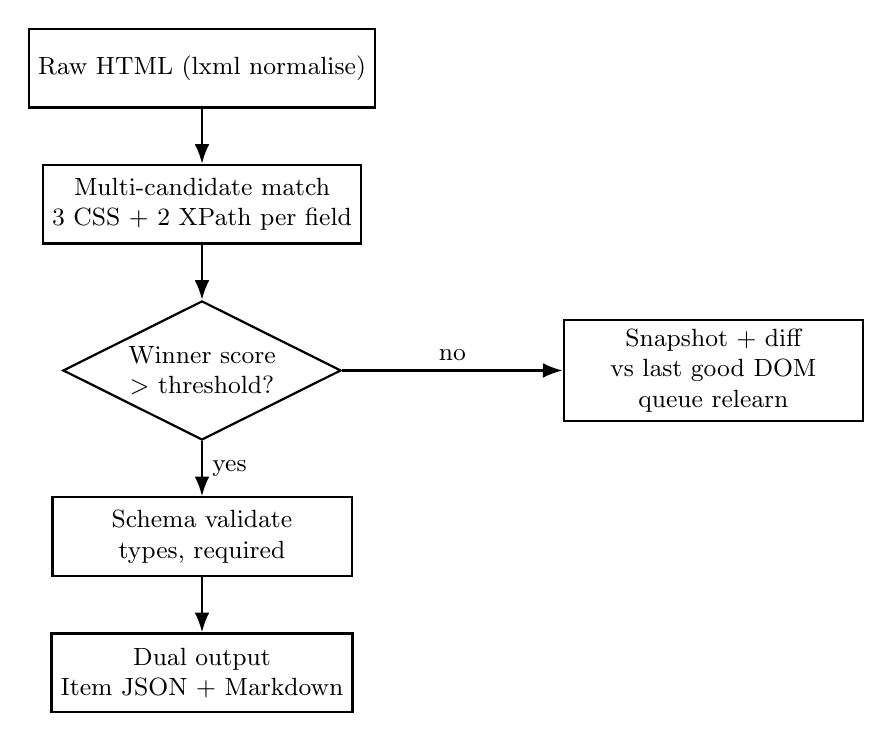
\begin{tikzpicture}[node distance=7mm]
\node[bwboxwide] (r) {Raw HTML (lxml normalise)};
\node[bwboxwide, below=of r] (m) {Multi-candidate match\\3 CSS + 2 XPath per field};
\node[bwdecision, below=of m] (s) {Winner score\\$>$ threshold?};
\node[bwboxwide, below=of s] (v) {Schema validate\\types, required};
\node[bwboxwide, below=of v] (o) {Dual output\\Item JSON + Markdown};
\node[bwboxwide, right=28mm of s] (l) {Snapshot + diff\\vs last good DOM\\queue relearn};
\draw[bwarrow] (r) -- (m);
\draw[bwarrow] (m) -- (s);
\draw[bwarrow] (s) -- node[right,font=\small]{yes} (v);
\draw[bwarrow] (v) -- (o);
\draw[bwarrow] (s) -- node[above,font=\small]{no} (l);
\end{tikzpicture}
\caption{Adaptive parse. Zero-match never drops silently; it snapshots for relearning.}
\label{fig:parser}
\end{figure}

Scoring inputs: candidate text density, DOM depth stability across samples, historical win rate stored in \texttt{selectors.yml}. Threshold default 0.65, tuned per spider.

% ============================================================
\section{Flow 4: Session and Proxy Lifecycle}
% ============================================================
\begin{figure}[H]
\centering
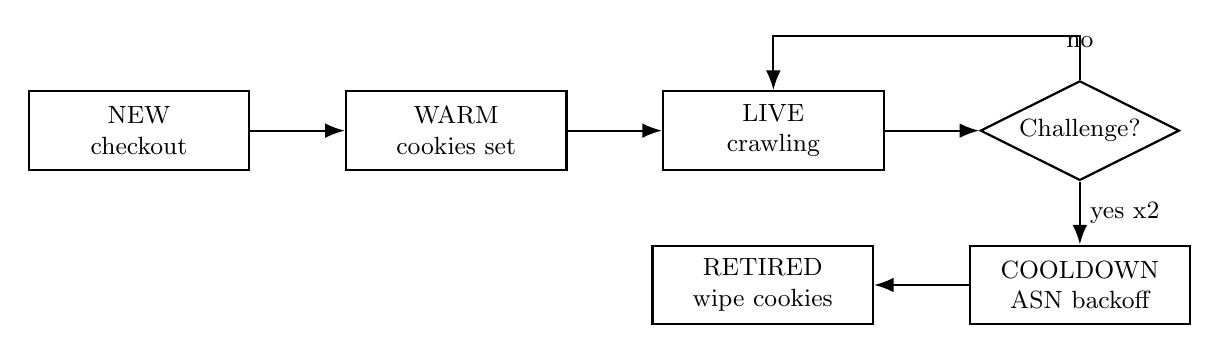
\begin{tikzpicture}[node distance=8mm and 12mm]
\node[bwbox] (new) {NEW\\checkout};
\node[bwbox, right=of new] (warm) {WARM\\cookies set};
\node[bwbox, right=of warm] (live) {LIVE\\crawling};
\node[bwdecision, right=of live] (chk) {Challenge?};
\node[bwbox, below=of chk] (cool) {COOLDOWN\\ASN backoff};
\node[bwbox, left=of cool] (ret) {RETIRED\\wipe cookies};
\draw[bwarrow] (new) -- (warm);
\draw[bwarrow] (warm) -- (live);
\draw[bwarrow] (live) -- (chk);
\draw[bwarrow] (chk) -- node[above,font=\small]{no} ++(0,12mm) -| (live);
\draw[bwarrow] (chk) -- node[right,font=\small]{yes x2} (cool);
\draw[bwarrow] (cool) -- (ret);
\end{tikzpicture}
\caption{Identity lifecycle. Two challenges retire the identity; cooldown protects the ASN pool.}
\label{fig:lifecycle}
\end{figure}

Proxy policy: residential exit per session; maximum 30 requests per IP per host per hour (tunable in \texttt{politeness.py}); health probe every 60\,s; failed ASN cooled for 15\,min.

% ============================================================
\section{Flow 5: Deployment View}
% ============================================================
\begin{figure}[H]
\centering
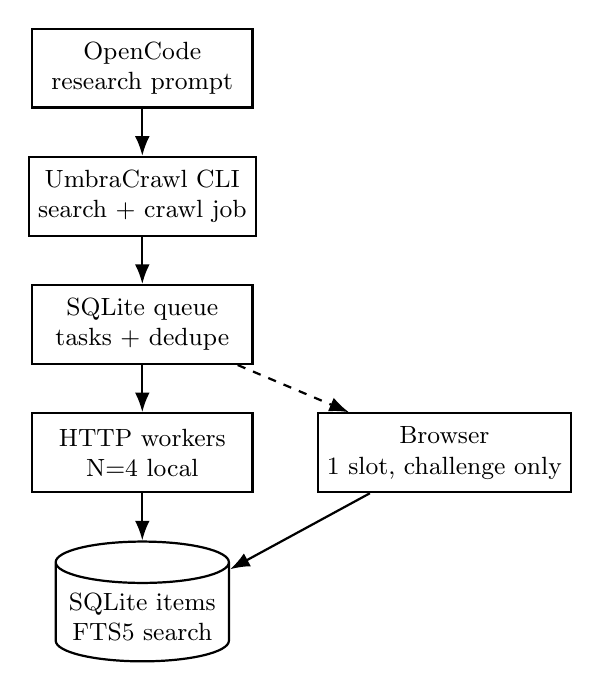
\begin{tikzpicture}[node distance=6mm and 8mm]
\node[bwbox] (op) {OpenCode\\research prompt};
\node[bwbox, below=of op] (cli) {UmbraCrawl CLI\\search + crawl job};
\node[bwbox, below=of cli] (q) {SQLite queue\\tasks + dedupe};
\node[bwbox, below=of q] (w1) {HTTP workers\\N=4 local};
\node[bwbox, right=of w1] (w2) {Browser\\1 slot, challenge only};
\node[bwdata, below=of w1] (store) {SQLite items\\FTS5 search};
\draw[bwarrow] (op) -- (cli);
\draw[bwarrow] (cli) -- (q);
\draw[bwarrow] (q) -- (w1);
\draw[bwdashed] (q) -- (w2);
\draw[bwarrow] (w1) -- (store);
\draw[bwarrow] (w2) -- (store);
\end{tikzpicture}
\caption{Local deployment. No servers: SQLite holds queue, dedupe, and items; the browser runs only on challenge.}
\label{fig:deploy}
\end{figure}

Local-first, single machine: 4 workers max against a SQLite task table (WAL mode). The browser borrows one of the 4 slots on challenge pages, so concurrency never exceeds 4. No Redis, no Postgres, nothing to deploy. The \texttt{storage/} interface stays abstract so a server backend can replace SQLite later without touching fetchers or parser.

% ============================================================
\section{Flow 6: Scheduler Queue Pipeline}
% ============================================================
\begin{figure}[H]
\centering
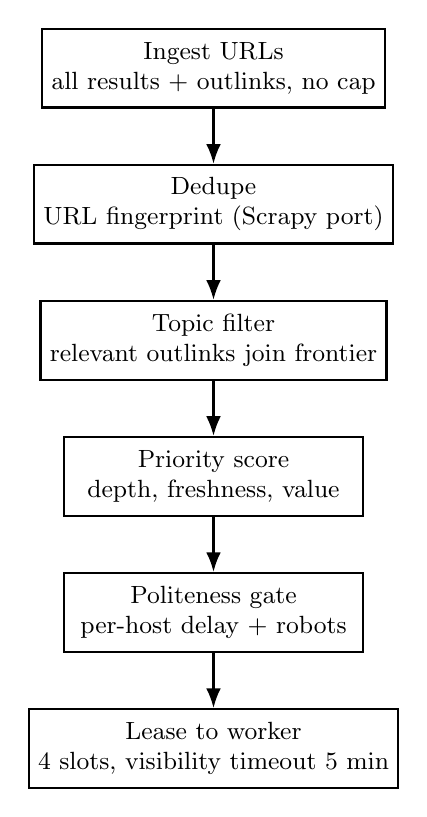
\begin{tikzpicture}[node distance=7mm]
\node[bwboxwide] (in) {Ingest URLs\\all results + outlinks, no cap};
\node[bwboxwide, below=of in] (dd) {Dedupe\\URL fingerprint (Scrapy port)};
\node[bwboxwide, below=of dd] (tf) {Topic filter\\relevant outlinks join frontier};
\node[bwboxwide, below=of tf] (pr) {Priority score\\depth, freshness, value};
\node[bwboxwide, below=of pr] (po) {Politeness gate\\per-host delay + robots};
\node[bwboxwide, below=of po] (le) {Lease to worker\\4 slots, visibility timeout 5 min};
\draw[bwarrow] (in) -- (dd);
\draw[bwarrow] (dd) -- (tf);
\draw[bwarrow] (tf) -- (pr);
\draw[bwarrow] (pr) -- (po);
\draw[bwarrow] (po) -- (le);
\end{tikzpicture}
\caption{Scheduler stages. Uncapped intake; a URL crawls only after dedupe, topic filter, scoring, and politeness all pass.}
\label{fig:scheduler}
\end{figure}

% ============================================================
\section{Flow 7: Challenge Detection Decision Tree}
% ============================================================
\begin{figure}[H]
\centering
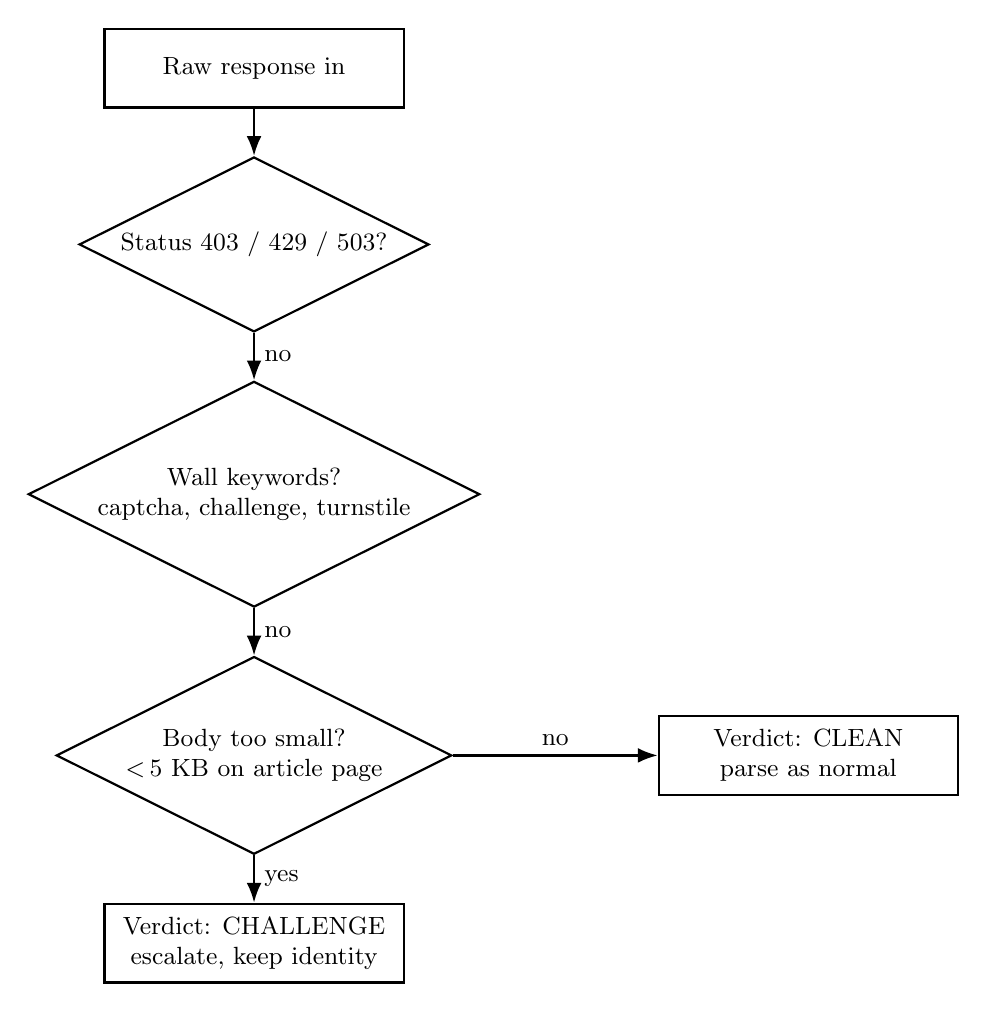
\begin{tikzpicture}[node distance=6mm]
\node[bwboxwide] (r) {Raw response in};
\node[bwdecision, below=of r] (s) {Status 403 / 429 / 503?};
\node[bwdecision, below=of s] (k) {Wall keywords?\\captcha, challenge, turnstile};
\node[bwdecision, below=of k] (b) {Body too small?\\\textless\,5 KB on article page};
\node[bwboxwide, below=of b] (v) {Verdict: CHALLENGE\\escalate, keep identity};
\node[bwboxwide, right=26mm of b] (c) {Verdict: CLEAN\\parse as normal};
\draw[bwarrow] (r) -- (s);
\draw[bwarrow] (s) -- node[right,font=\small]{no} (k);
\draw[bwarrow] (k) -- node[right,font=\small]{no} (b);
\draw[bwarrow] (b) -- node[right,font=\small]{yes} (v);
\draw[bwarrow] (b) -- node[above,font=\small]{no} (c);
\end{tikzpicture}
\caption{Challenge detector. Any yes on the three tests routes to the browser path.}
\label{fig:challenge}
\end{figure}

% ============================================================
\section{Flow 8: Fingerprint Assembly}
% ============================================================
\begin{figure}[H]
\centering
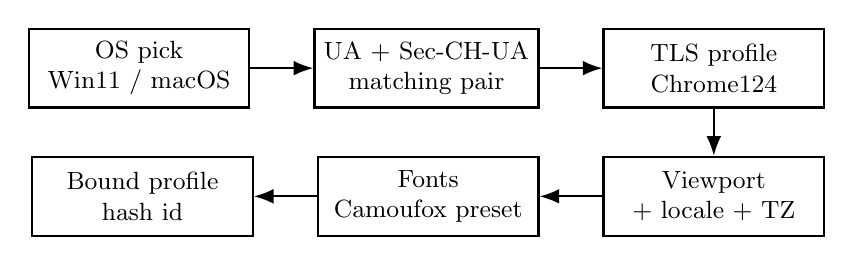
\begin{tikzpicture}[node distance=6mm and 8mm]
\node[bwbox] (os) {OS pick\\Win11 / macOS};
\node[bwbox, right=of os] (ua) {UA + Sec-CH-UA\\matching pair};
\node[bwbox, right=of ua] (tls) {TLS profile\\Chrome124};
\node[bwbox, below=of tls] (vp) {Viewport\\+ locale + TZ};
\node[bwbox, left=of vp] (fo) {Fonts\\Camoufox preset};
\node[bwbox, left=of fo] (out) {Bound profile\\hash id};
\draw[bwarrow] (os) -- (ua);
\draw[bwarrow] (ua) -- (tls);
\draw[bwarrow] (tls) -- (vp);
\draw[bwarrow] (vp) -- (fo);
\draw[bwarrow] (fo) -- (out);
\end{tikzpicture}
\caption{Fingerprint assembly. Every field derives from one OS choice so the profile stays self-consistent.}
\label{fig:fingerprint}
\end{figure}

% ============================================================
\section{Flow 9: Proxy Health Loop}
% ============================================================
\begin{figure}[H]
\centering
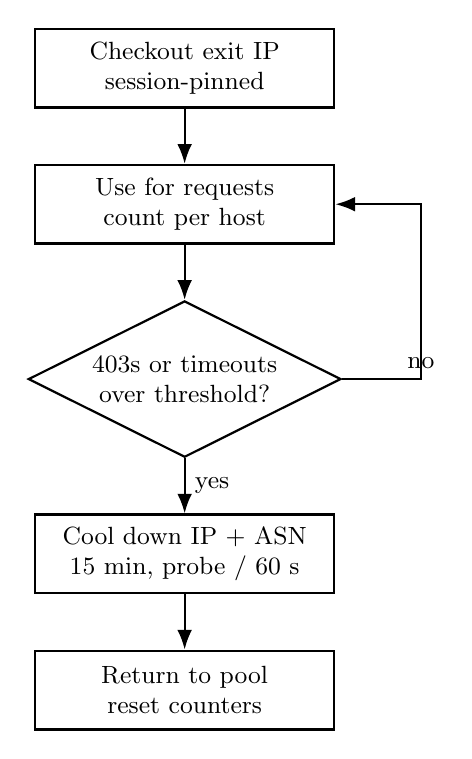
\begin{tikzpicture}[node distance=7mm]
\node[bwboxwide] (ck) {Checkout exit IP\\session-pinned};
\node[bwboxwide, below=of ck] (use) {Use for requests\\count per host};
\node[bwdecision, below=of use] (ok) {403s or timeouts\\over threshold?};
\node[bwboxwide, below=of ok] (cool) {Cool down IP + ASN\\15 min, probe / 60 s};
\node[bwboxwide, below=of cool] (back) {Return to pool\\reset counters};
\draw[bwarrow] (ck) -- (use);
\draw[bwarrow] (use) -- (ok);
\draw[bwarrow] (ok) -- node[right,font=\small]{yes} (cool);
\draw[bwarrow] (cool) -- (back);
\draw[bwarrow] (ok) -| node[above,font=\small]{no} ++(30mm,0) |- (use);
\end{tikzpicture}
\caption{Proxy health loop. Failures cool the IP and its ASN together to stop cluster-wide burns.}
\label{fig:proxy}
\end{figure}

% ============================================================
\section{Flow 10: Browser Pool Manager}
% ============================================================
\begin{figure}[H]
\centering
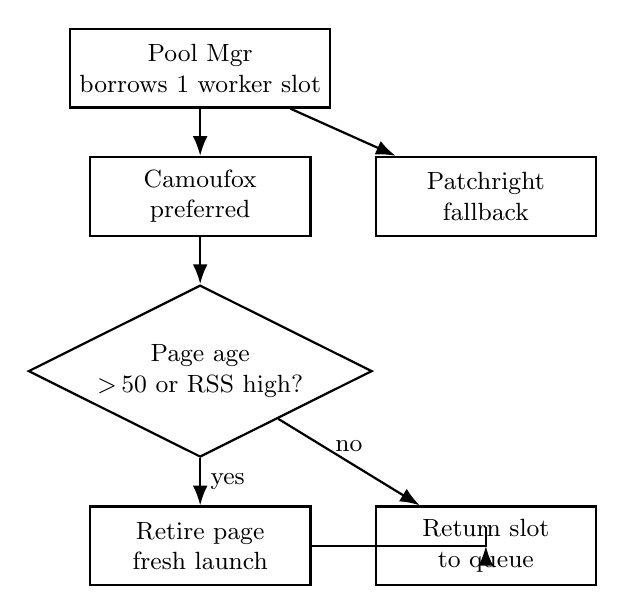
\begin{tikzpicture}[node distance=6mm and 8mm]
\node[bwbox] (mgr) {Pool Mgr\\borrows 1 worker slot};
\node[bwbox, below=of mgr] (cx) {Camoufox\\preferred};
\node[bwbox, right=of cx] (pr) {Patchright\\fallback};
\node[bwdecision, below=of cx] (age) {Page age\\\textgreater\,50 or RSS high?};
\node[bwbox, below=of age] (ret) {Retire page\\fresh launch};
\node[bwbox, right=of ret] (q) {Return slot\\to queue};
\draw[bwarrow] (mgr) -- (cx);
\draw[bwarrow] (mgr) -- (pr);
\draw[bwarrow] (cx) -- (age);
\draw[bwarrow] (age) -- node[right,font=\small]{yes} (ret);
\draw[bwarrow] (age) -- node[above,font=\small]{no} (q);
\draw[bwarrow] (ret) -| (q);
\end{tikzpicture}
\caption{Browser slot. One worker slot converts to a browser page on challenge; the other three keep crawling.}
\label{fig:pool}
\end{figure}

% ============================================================
\section{Flow 11: Leak Check Suite}
% ============================================================
\begin{figure}[H]
\centering
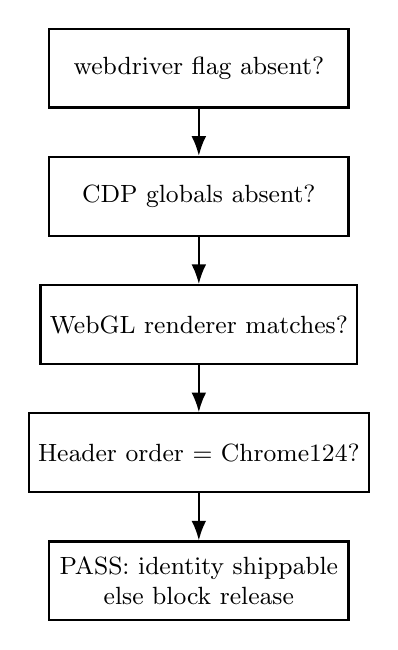
\begin{tikzpicture}[node distance=6mm]
\node[bwboxwide] (w) {webdriver flag absent?};
\node[bwboxwide, below=of w] (c) {CDP globals absent?};
\node[bwboxwide, below=of c] (g) {WebGL renderer matches?};
\node[bwboxwide, below=of g] (h) {Header order = Chrome124?};
\node[bwboxwide, below=of h] (p) {PASS: identity shippable\\else block release};
\draw[bwarrow] (w) -- (c);
\draw[bwarrow] (c) -- (g);
\draw[bwarrow] (g) -- (h);
\draw[bwarrow] (h) -- (p);
\end{tikzpicture}
\caption{Leak gate. Ported from Patchright smoke test; a new profile ships only after all four pass.}
\label{fig:leak}
\end{figure}

% ============================================================
\section{Flow 12: Pipeline Validation Chain}
% ============================================================
\begin{figure}[H]
\centering
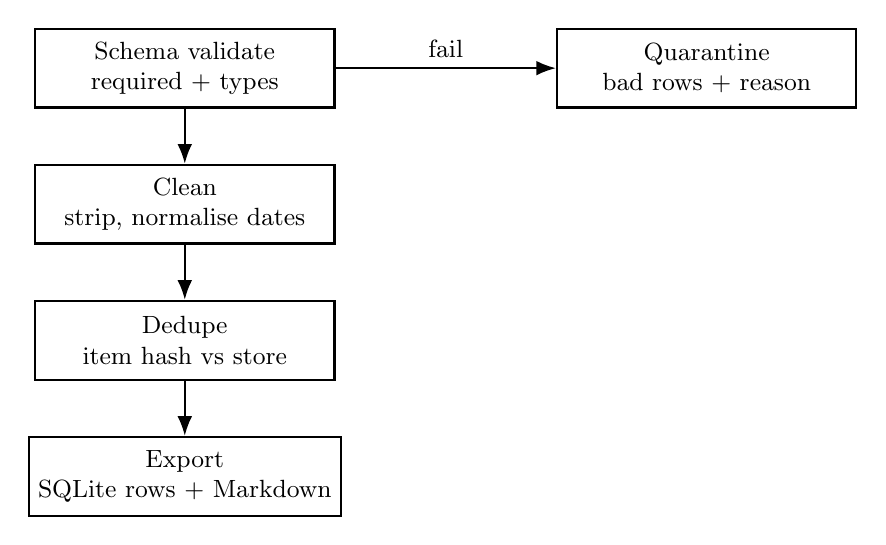
\begin{tikzpicture}[node distance=7mm]
\node[bwboxwide] (v) {Schema validate\\required + types};
\node[bwboxwide, below=of v] (cl) {Clean\\strip, normalise dates};
\node[bwboxwide, below=of cl] (dd) {Dedupe\\item hash vs store};
\node[bwboxwide, below=of dd] (ex) {Export\\SQLite rows + Markdown};
\node[bwboxwide, right=28mm of v] (qu) {Quarantine\\bad rows + reason};
\draw[bwarrow] (v) -- (cl);
\draw[bwarrow] (cl) -- (dd);
\draw[bwarrow] (dd) -- (ex);
\draw[bwarrow] (v) -- node[above,font=\small]{fail} (qu);
\end{tikzpicture}
\caption{Export pipeline. Failures quarantine with reasons; good rows fan out to both stores.}
\label{fig:pipeline}
\end{figure}

% ============================================================
\section{Flow 13: Local Run Sequence (CLI)}
% ============================================================
\begin{figure}[H]
\centering
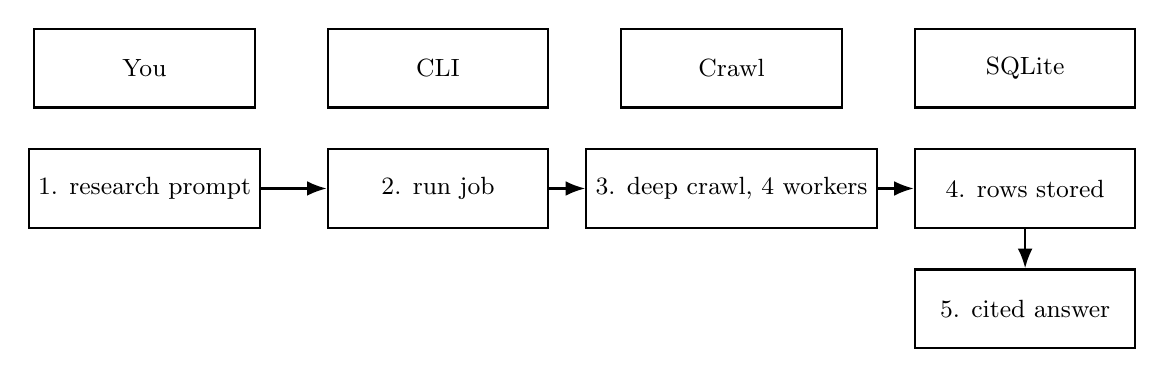
\begin{tikzpicture}[node distance=5mm and 9mm]
\node[bwbox] (cl) {You};
\node[bwbox, right=of cl] (gw) {CLI};
\node[bwbox, right=of gw] (sc) {Crawl};
\node[bwbox, right=of sc] (wh) {SQLite};
\node[bwbox, below=of cl] (a) {1. research prompt};
\node[bwbox, below=of gw] (b) {2. run job};
\node[bwbox, below=of sc] (c) {3. deep crawl, 4 workers};
\node[bwbox, below=of wh] (d) {4. rows stored};
\node[bwbox, below=of d] (e) {5. cited answer};
\draw[bwarrow] (a) -- (b);
\draw[bwarrow] (b) -- (c);
\draw[bwarrow] (c) -- (d);
\draw[bwarrow] (d) -- (e);
\end{tikzpicture}
\caption{Local run contract: prompt in, deep crawl on 4 workers, cited answer out. No servers, no webhooks.}
\label{fig:localrun}
\end{figure}

% ============================================================
\section{Flow 14: Retry Budget and Error Handling}
% ============================================================
\begin{figure}[H]
\centering
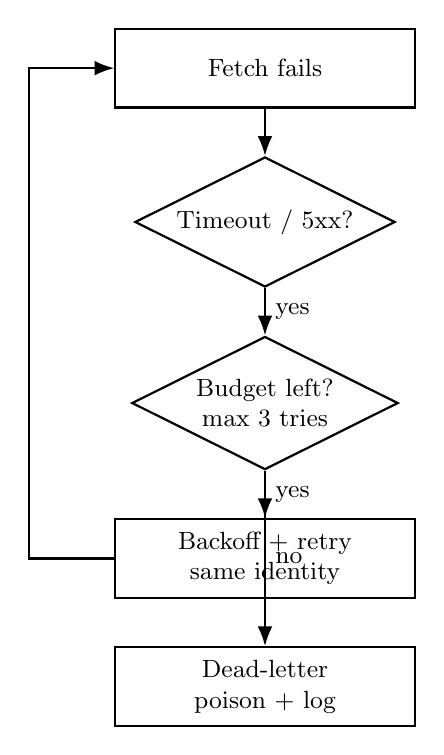
\begin{tikzpicture}[node distance=6mm]
\node[bwboxwide] (f) {Fetch fails};
\node[bwdecision, below=of f] (t) {Timeout / 5xx?};
\node[bwdecision, below=of t] (b) {Budget left?\\max 3 tries};
\node[bwboxwide, below=of b] (w) {Backoff + retry\\same identity};
\node[bwboxwide, below=of w] (d) {Dead-letter\\poison + log};
\draw[bwarrow] (f) -- (t);
\draw[bwarrow] (t) -- node[right,font=\small]{yes} (b);
\draw[bwarrow] (b) -- node[right,font=\small]{yes} (w);
\draw[bwarrow] (w) -| ++(-30mm,0) |- (f);
\draw[bwarrow] (b) -- node[right,font=\small]{no} (d);
\end{tikzpicture}
\caption{Retry budget. Only transient errors retry; challenges leave this loop for the escalation path.}
\label{fig:retry}
\end{figure}

% ============================================================
\section{Flow 15: Selector Relearn Loop}
% ============================================================
\begin{figure}[H]
\centering
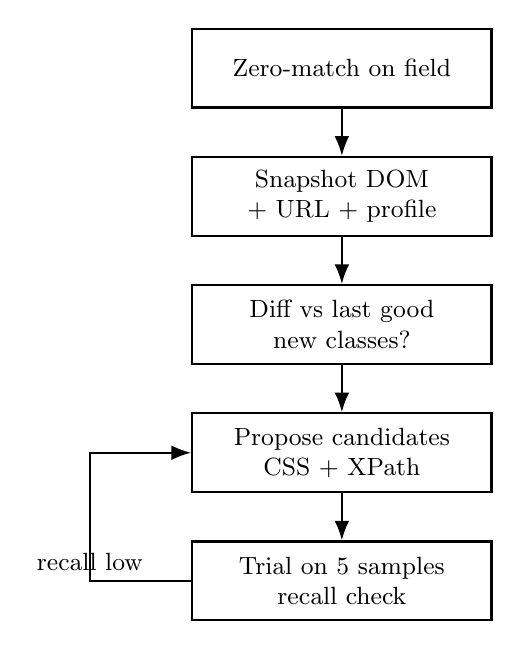
\begin{tikzpicture}[node distance=6mm]
\node[bwboxwide] (z) {Zero-match on field};
\node[bwboxwide, below=of z] (s) {Snapshot DOM\\+ URL + profile};
\node[bwboxwide, below=of s] (d) {Diff vs last good\\new classes?};
\node[bwboxwide, below=of d] (c) {Propose candidates\\CSS + XPath};
\node[bwboxwide, below=of c] (t) {Trial on 5 samples\\recall check};
\draw[bwarrow] (z) -- (s);
\draw[bwarrow] (s) -- (d);
\draw[bwarrow] (d) -- (c);
\draw[bwarrow] (c) -- (t);
\draw[bwarrow] (t) -| node[above,font=\small]{recall low} ++(-32mm,0) |- (c);
\end{tikzpicture}
\caption{Relearn detail for Figure~\ref{fig:parser}. Candidates graduate to \texttt{selectors.yml} only after trials.}
\label{fig:relearn}
\end{figure}

% ============================================================
\section{Flow 16: Data Model}
% ============================================================
\begin{figure}[H]
\centering
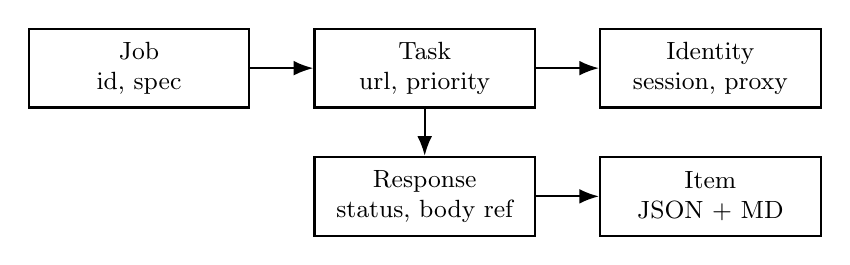
\begin{tikzpicture}[node distance=6mm and 8mm]
\node[bwbox] (job) {Job\\id, spec};
\node[bwbox, right=of job] (task) {Task\\url, priority};
\node[bwbox, right=of task] (iden) {Identity\\session, proxy};
\node[bwbox, below=of task] (resp) {Response\\status, body ref};
\node[bwbox, right=of resp] (item) {Item\\JSON + MD};
\draw[bwarrow] (job) -- (task);
\draw[bwarrow] (task) -- (iden);
\draw[bwarrow] (task) -- (resp);
\draw[bwarrow] (resp) -- (item);
\end{tikzpicture}
\caption{Core records. One job owns many tasks; each task binds one identity and yields one response.}
\label{fig:datamodel}
\end{figure}

% ============================================================
\section{Flow 17: Observability and Autoscale}
% ============================================================
\begin{figure}[H]
\centering
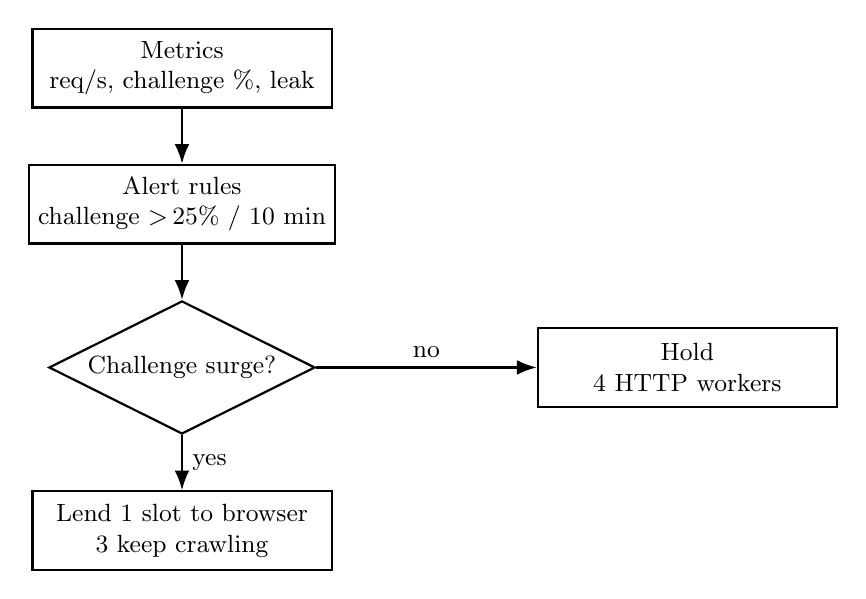
\begin{tikzpicture}[node distance=7mm]
\node[bwboxwide] (m) {Metrics\\req/s, challenge \%, leak};
\node[bwboxwide, below=of m] (a) {Alert rules\\challenge \textgreater\,25\% / 10 min};
\node[bwdecision, below=of a] (s) {Challenge surge?};
\node[bwboxwide, below=of s] (up) {Lend 1 slot to browser\\3 keep crawling};
\node[bwboxwide, right=28mm of s] (hold) {Hold\\4 HTTP workers};
\draw[bwarrow] (m) -- (a);
\draw[bwarrow] (a) -- (s);
\draw[bwarrow] (s) -- node[right,font=\small]{yes} (up);
\draw[bwarrow] (s) -- node[above,font=\small]{no} (hold);
\end{tikzpicture}
\caption{Control loop. Fixed 4-worker budget: challenge surges only move a slot to the browser, never add workers.}
\label{fig:observe}
\end{figure}

% ============================================================
\section{Flow 18: Threat Coverage Map}
% ============================================================
\begin{figure}[H]
\centering
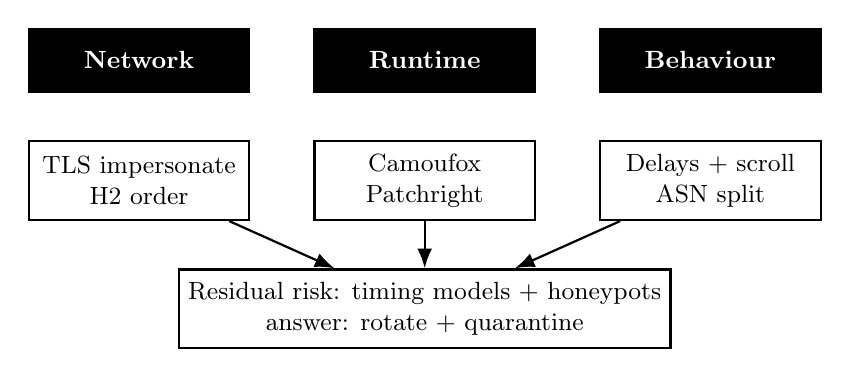
\begin{tikzpicture}[node distance=6mm and 8mm]
\node[bwheader] (n) {Network};
\node[bwheader, right=of n] (r) {Runtime};
\node[bwheader, right=of r] (b) {Behaviour};
\node[bwbox, below=of n] (n1) {TLS impersonate\\H2 order};
\node[bwbox, below=of r] (r1) {Camoufox\\Patchright};
\node[bwbox, below=of b] (b1) {Delays + scroll\\ASN split};
\node[bwboxwide, below=of r1] (all) {Residual risk: timing models + honeypots\\answer: rotate + quarantine};
\draw[bwarrow] (n1) -- (all);
\draw[bwarrow] (r1) -- (all);
\draw[bwarrow] (b1) -- (all);
\end{tikzpicture}
\caption{Coverage map. Each adversary signal class has one owning defence; residuals are handled by rotation.}
\label{fig:threat}
\end{figure}

% ============================================================
\section{Flow 19: Versioned Build Phases}
% ============================================================
\begin{figure}[H]
\centering
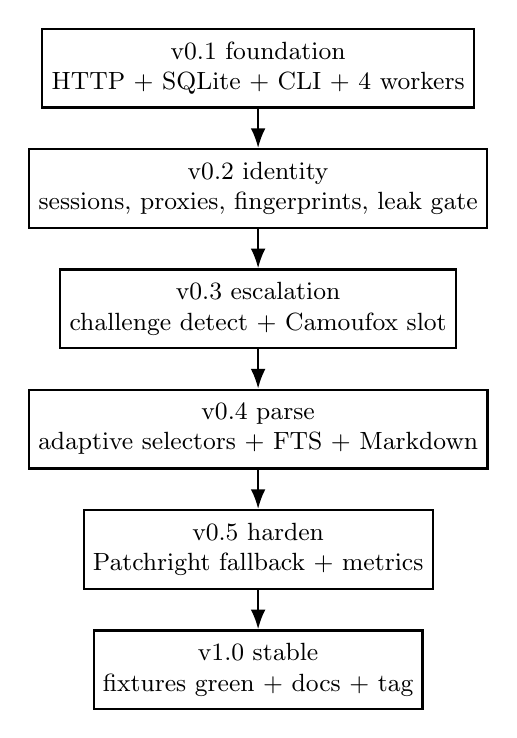
\begin{tikzpicture}[node distance=5mm]
\node[bwboxwide] (p1) {v0.1 foundation\\HTTP + SQLite + CLI + 4 workers};
\node[bwboxwide, below=of p1] (p2) {v0.2 identity\\sessions, proxies, fingerprints, leak gate};
\node[bwboxwide, below=of p2] (p3) {v0.3 escalation\\challenge detect + Camoufox slot};
\node[bwboxwide, below=of p3] (p4) {v0.4 parse\\adaptive selectors + FTS + Markdown};
\node[bwboxwide, below=of p4] (p5) {v0.5 harden\\Patchright fallback + metrics};
\node[bwboxwide, below=of p5] (p6) {v1.0 stable\\fixtures green + docs + tag};
\draw[bwarrow] (p1) -- (p2);
\draw[bwarrow] (p2) -- (p3);
\draw[bwarrow] (p3) -- (p4);
\draw[bwarrow] (p4) -- (p5);
\draw[bwarrow] (p5) -- (p6);
\end{tikzpicture}
\caption{Version ladder. Each version ships a working researcher; nothing lands half-wired.}
\label{fig:phases}
\end{figure}

% ============================================================
\section{Flow 20: Local Research Loop (OpenCode)}
% ============================================================
Your use case, end to end. You type \texttt{research a book} in OpenCode; UmbraCrawl does the legwork and hands structured rows back for the answer. No page cap: it works the full frontier for as long as it takes, on 4 workers.

\begin{figure}[H]
\centering
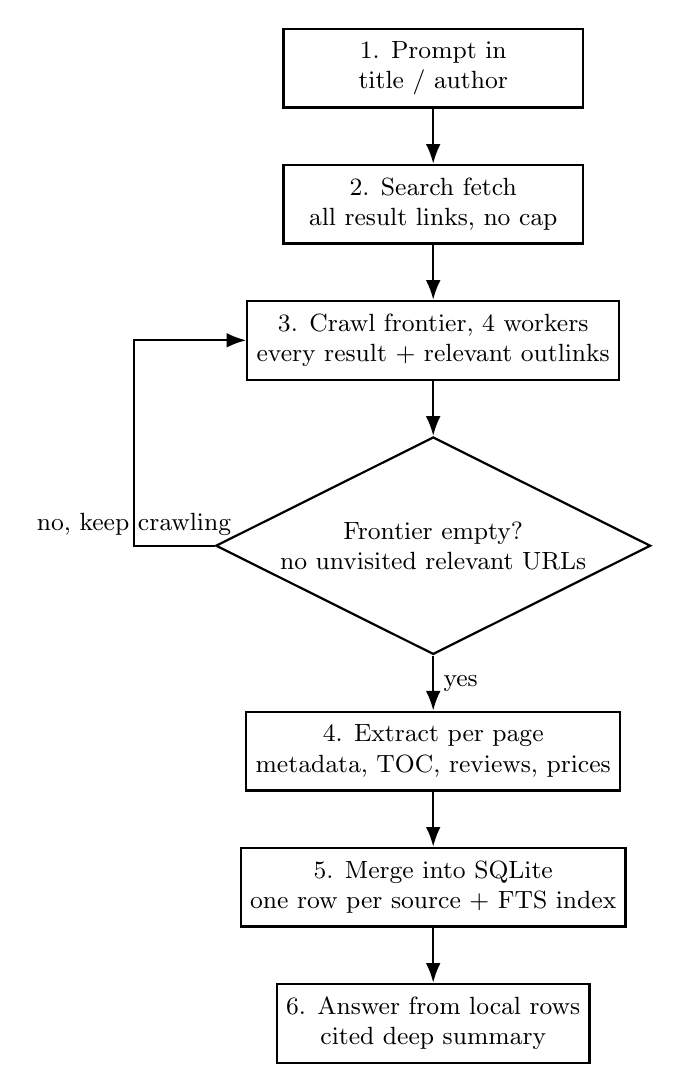
\begin{tikzpicture}[node distance=7mm]
\node[bwboxwide] (p) {1. Prompt in\\title / author};
\node[bwboxwide, below=of p] (s) {2. Search fetch\\all result links, no cap};
\node[bwboxwide, below=of s] (c) {3. Crawl frontier, 4 workers\\every result + relevant outlinks};
\node[bwdecision, below=of c] (f) {Frontier empty?\\no unvisited relevant URLs};
\node[bwboxwide, below=of f] (e) {4. Extract per page\\metadata, TOC, reviews, prices};
\node[bwboxwide, below=of e] (m) {5. Merge into SQLite\\one row per source + FTS index};
\node[bwboxwide, below=of m] (a) {6. Answer from local rows\\cited deep summary};
\draw[bwarrow] (p) -- (s);
\draw[bwarrow] (s) -- (c);
\draw[bwarrow] (c) -- (f);
\draw[bwarrow] (f) -- node[right,font=\small]{yes} (e);
\draw[bwarrow] (f) -| node[above,font=\small]{no, keep crawling} ++(-38mm,0) |- (c);
\draw[bwarrow] (e) -- (m);
\draw[bwarrow] (m) -- (a);
\end{tikzpicture}
\caption{Research loop. Uncapped: the frontier drains fully before extraction merges and the answer composes.}
\label{fig:research}
\end{figure}

Depth rules: every search result is crawled, and each page's outlinks join the frontier when they match the topic filter (same book, author, publisher, reviews). Only 4 workers run at a time; time is unbounded. Repeat queries hit SQLite first: if the book's sources are already stored and fresh, step~6 answers with zero network. Stale rows (older than the freshness window in \texttt{politeness.py}) re-queue only their URLs.

% ============================================================
\section{Stealth Matrix}
% ============================================================
\begin{table}[H]
\centering
\caption{Technique versus signal. B/W print: pass = closed square, partial = half, fail = open (described in text).}
\begin{tabular}{@{}p{4cm}p{4cm}p{5.6cm}@{}}
\toprule
Technique & Defeats & Caught by \\
\midrule
TLS + H2 impersonation (\texttt{curl\_cffi}) & JA3 / header-order filters & JS challenges, Turnstile. \\
Camoufox engine patches & Canvas, font, WebGL, \texttt{webdriver} checks & Behavioural timing, mouse entropy. \\
Patchright CDP patches & CDP command probes (Cloudflare) & Version drift if unpatched. \\
Residential rotation + ASN split & IP rate limits, ASN bans & Cost; still needs politeness. \\
Humanised behaviour (scroll, dwell) & Headless heuristics & Long-run timing models. \\
\bottomrule
\end{tabular}
\end{table}

% ============================================================
\section{Verification Plan}
% ============================================================
\begin{enumerate}[leftmargin=*,itemsep=3pt]
\item \textbf{Leak suite} (\texttt{tests/leak\_suite.py}, from Patchright smoke test): assert \texttt{navigator.webdriver} undefined, CDP globals absent, WebGL renderer matches profile, headers order matches Chrome124.
\item \textbf{Challenge fixtures}: recorded Cloudflare / DataDome pages; assert router escalates and recovers body $>$ 5\,KB.
\item \textbf{Parse recall}: per-field precision/recall on 50 sampled pages; assert recall $\geq$ 0.95 after relearn.
\item \textbf{Ban metrics}: challenge rate, 403 share, proxy retry share, ASN cooldown events; alert if challenge rate $>$ 25\% over 10\,min.
\item \textbf{Load test}: 4 workers against local fixtures; record pages/min and p95 fetch latency.
\end{enumerate}

% ============================================================
\section{Build Order: v0.1 to v1.0}
% ============================================================
\begin{enumerate}[leftmargin=*,itemsep=3pt]
\item \textbf{v0.1 foundation.} HTTP fetcher (\texttt{curl\_cffi}), SQLite task/item tables, scheduler with dedupe + politeness, CLI research loop uncapped on 4 workers. Done when a book prompt returns cited rows.
\item \textbf{v0.2 identity.} Sessions, proxy support, \texttt{browserforge} fingerprints, leak gate (Figure~\ref{fig:leak}). Done when all four leak checks pass.
\item \textbf{v0.3 escalation.} Challenge detector (Figure~\ref{fig:challenge}) + router + Camoufox borrowed slot (Figure~\ref{fig:pool}). Done when fixtures recover bodies $>$ 5\,KB.
\item \textbf{v0.4 parse.} Adaptive multi-candidate selectors, relearn loop (Figure~\ref{fig:relearn}), FTS5 index, Markdown output. Done when recall $\geq$ 0.95 on samples.
\item \textbf{v0.5 harden.} Patchright fallback, proxy cooldowns, metrics + alerts. Done when challenge rate $<$ 25\% on test set.
\item \textbf{v1.0 stable.} Fixture suite green, docs complete, version tag cut. No new features; only fixes.
\end{enumerate}

\end{document}
